%%%%%%%%%%%%
%
% $Autor: Alexandra $
% $Datum: 2026-06-22 $
% $Pfad: HotWire/report/Contents/General $
% !TeX spellcheck = de_DE
% !TeX encoding = utf8
% !TeX root = ../../System/EdgeComputer/filename.tex
% !TeX TXS-program:bibliography = txs:///biber
%
%%%%%%%%%%%%

% Structure
\chapter{Universal G-Code Sender}
\label{cha:ugs}

\section{Einleitung}

Dieses Kapitel beschreibt den Universal G-Code Sender, kurz UGS, als Bediensoftware für GRBL-basierte CNC-Systeme. Die Software stellt die Verbindung zwischen dem Computer und dem Mikrocontroller her, lädt G-Code-Dateien, visualisiert Werkzeugpfade und überträgt die Befehle zeilenweise an die Steuerung. Damit bildet UGS die Benutzeroberfläche des Heißdraht Schneiders, während GRBL die Bewegungsbefehle auf dem Arduino verarbeitet.

\section{Beschreibung des Universal G-Code Senders}

Der Universal G-Code Sender ist eine quelloffene, Java-basierte Steuerungssoftware zur seriellen Kommunikation zwischen einem Host-Computer und dem Mikrocontroller einer CNC-Maschine. UGS ist plattformübergreifend und kann unter anderem unter Windows, Linux und macOS verwendet werden. Die Software bündelt die notwendigen Laufzeitkomponenten in einem ausführbaren Paket und kann dadurch ohne separat installierte Java-Laufzeitumgebung genutzt werden \cite{ugs:github}.

UGS übernimmt im Betrieb mehrere zentrale Aufgaben:

\begin{itemize}
	\item Kommunikationsschicht: Verwaltung der seriellen Verbindung über USB einschließlich Portauswahl, Baudrateneinstellung und Puffersteuerung.
	\item G-Code-Sender: Laden, Prüfen und zeilenweises Übertragen von G-Code-Dateien an den Controller.
	\item Maschinenzustandsanzeige: Darstellung des aktuellen Zustands, der Achspositionen und weiterer Steuerungsinformationen im Digital Read-Out.
	\item Werkzeugpfad-Visualisierung: Grafische Vorschau des geladenen G-Codes in einer 2D- beziehungsweise 3D-Ansicht.
	\item Konsolenzugriff: Direkte Eingabe einzelner Befehle und Anzeige von Rückmeldungen der Firmware.
\end{itemize}

Die Anwendungsbereiche von UGS umfassen Maschinen, die G-Code-basierte Steuerbefehle verarbeiten. Dazu gehören CNC-Fräsmaschinen, Laserschneider, Lasergraviermaschinen, Plotter und andere kartesische Bewegungssysteme \cite{ugs:github}.

\section{Aufbau der Benutzeroberfläche}

Die Benutzeroberfläche von UGS ist in mehrere Funktionsbereiche gegliedert. Diese Trennung erleichtert die Bedienung, weil Maschinenzustand, manuelle Steuerung, Werkzeugpfad-Vorschau und Diagnose voneinander getrennt dargestellt werden. Für die praktische Anwendung sind besonders die Bereiche \emph{Jog Control}, \emph{Visualizer}, \emph{Console} und \emph{Controller State / DRO} wichtig \cite{ugs:github}.

\subsection{Jog Control}

Die Jog Control dient zur manuellen Bewegung der Achsen. Mit ihrer Hilfe kann die Maschine schrittweise in positive oder negative Richtung verfahren werden. Dies ist zum Beispiel notwendig, um den Werkstücknullpunkt anzufahren, die Achsrichtung zu prüfen oder die Maschine vor einem Bearbeitungsvorgang zu positionieren.

Typische Anwendungsfälle der Jog-Steuerung sind:

\begin{itemize}
	\item Anfahren des Werkstücknullpunkts,
	\item Test der Achsbewegungen nach dem Verbindungsaufbau,
	\item Verfahren zu Referenz- oder Prüfpositionen,
	\item Kontrolle der richtigen Bewegungsrichtung einzelner Achsen.
\end{itemize}

\begin{figure}[H]
	\centering
	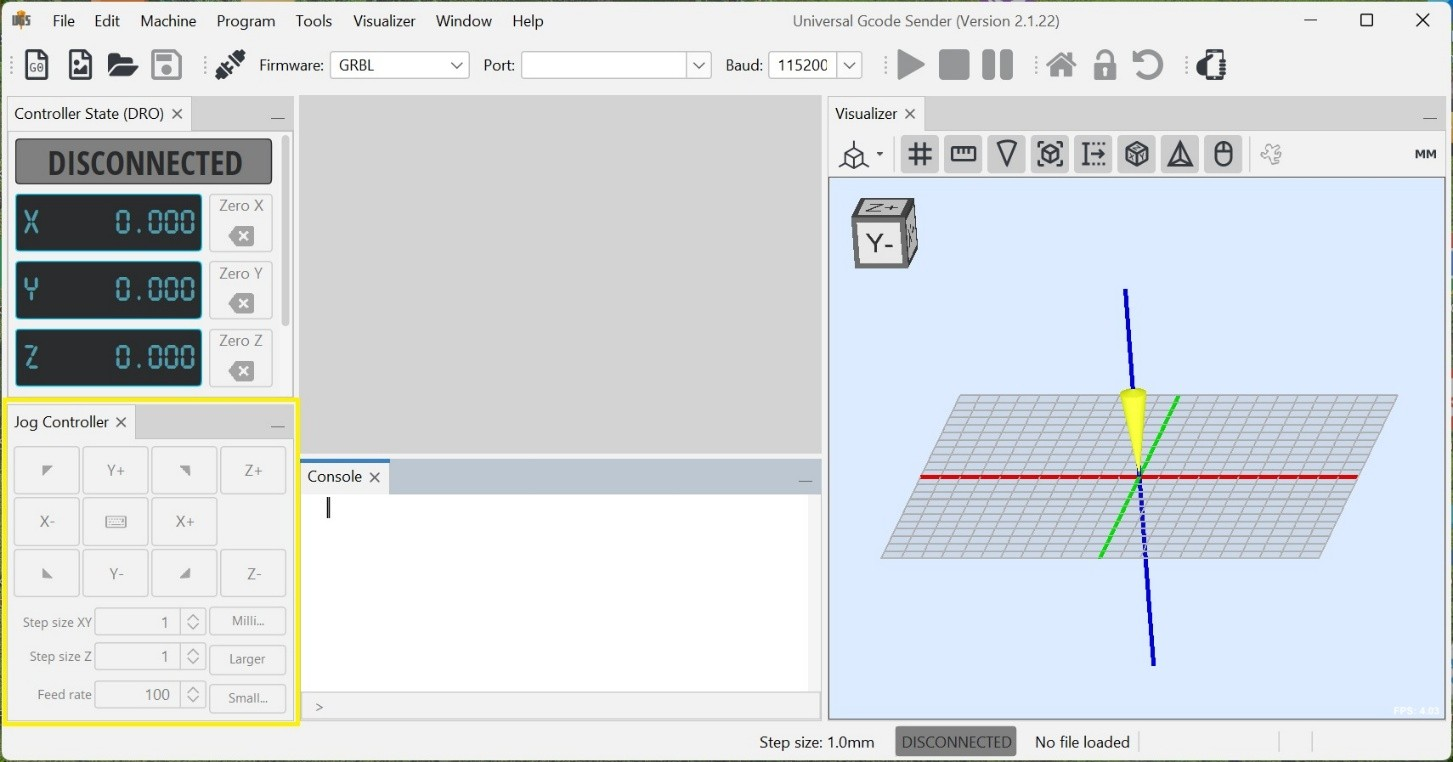
\includegraphics[width=0.85\linewidth]{../../Images/UGS/UGS_Jog_Control}
	\caption{Jog Control -- Bedienfeld in UGS}
	\label{fig:ugs_jog_control}
\end{figure}

\subsection{Visualizer}

Der Visualizer dient der grafischen Darstellung des geladenen G-Code-Programms. In diesem Fenster wird die Werkzeugbahn als 2D- oder 3D-Vorschau angezeigt. Dadurch kann vor dem Start geprüft werden, ob die Kontur, die Bewegungsrichtung und die Ausrichtung des Programms plausibel sind.

Der Visualizer unterstützt insbesondere:

\begin{itemize}
	\item die Kontrolle der importierten Werkzeugbahn,
	\item die Erkennung fehlerhafter Konturen oder unerwarteter Verfahrwege,
	\item die Darstellung der aktuellen Werkzeugposition während der Bearbeitung,
	\item die Überprüfung von Start- und Zielpunkten.
\end{itemize}

\begin{figure}[H]
	\centering
	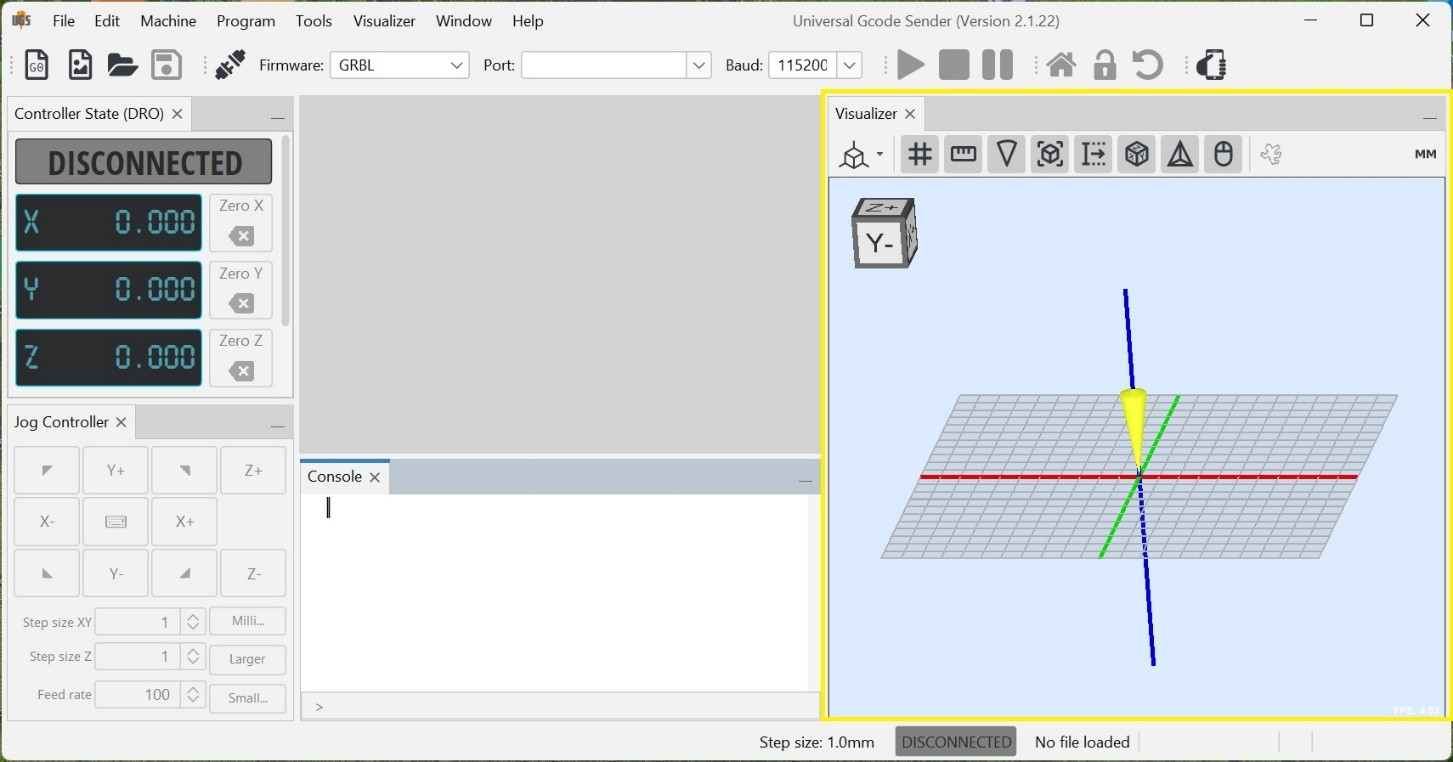
\includegraphics[width=0.85\linewidth]{../../Images/UGS/UGS_Visualizer}
	\caption{Visualizer -- Grafikanzeigefeld in UGS}
	\label{fig:ugs_visualizer}
\end{figure}

\subsection{Console}

Die Console ist die textbasierte Kommunikationsschnittstelle zwischen UGS und der Firmware. In diesem Bereich werden gesendete Befehle, empfangene Rückmeldungen, Statusmeldungen und Fehlermeldungen angezeigt. Sie ist deshalb ein wichtiges Werkzeug für Diagnose, Konfiguration und Fehlersuche \cite{ugs:github}.

Über die Console können einzelne Befehle direkt eingegeben werden, zum Beispiel:

\begin{itemize}
	\item \PYTHON{\$\$} zum Anzeigen aller gespeicherten GRBL-Parameter,
	\item \PYTHON{\$G} zum Anzeigen der aktiven modalen Zustände,
	\item \PYTHON{?} zur Statusabfrage,
	\item \PYTHON{\$H} zum Starten des Homing-Zyklus,
	\item \PYTHON{\$X} zum Entsperren nach einem Alarmzustand.
\end{itemize}

\begin{figure}[H]
	\centering
	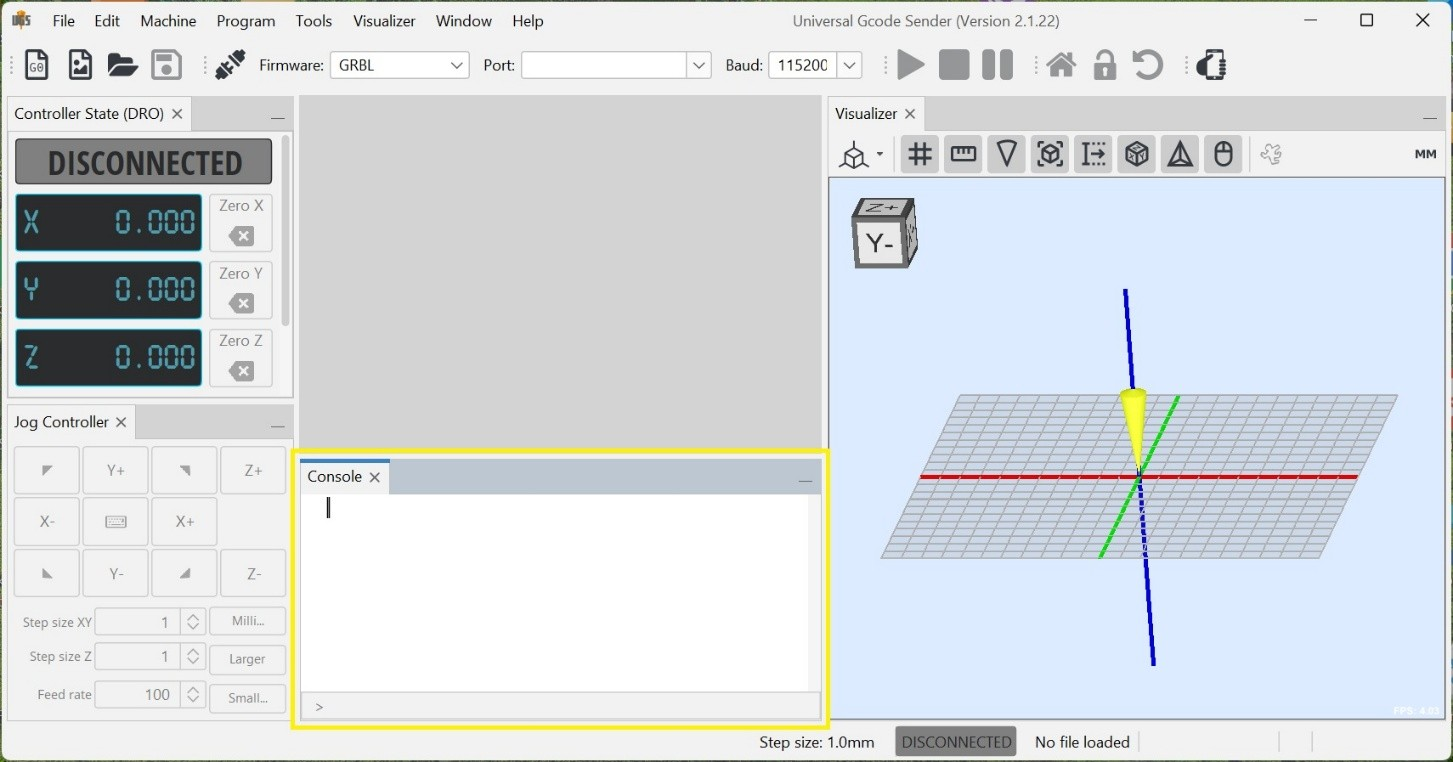
\includegraphics[width=0.85\linewidth]{../../Images/UGS/UGS_Console}
	\caption{Console -- Eingabefeld in UGS}
	\label{fig:ugs_console}
\end{figure}

\subsection{Controller State / DRO}

Der Bereich Controller State, häufig auch als DRO (Digital Read-Out) bezeichnet, zeigt den aktuellen Maschinenzustand in Echtzeit an. Dort werden die aktuellen Koordinaten der Achsen sowie Zustände wie \PYTHON{Idle}, \PYTHON{Run}, \PYTHON{Hold} oder \PYTHON{Alarm} angezeigt.

Dieser Bereich dient zur Kontrolle der aktuellen Achspositionen, zur Überwachung des Maschinenzustands, zur Prüfung des Werkstücknullpunkts und zur Rückmeldung über laufende oder fehlerhafte Bewegungsabläufe.

\begin{figure}[H]
	\centering
	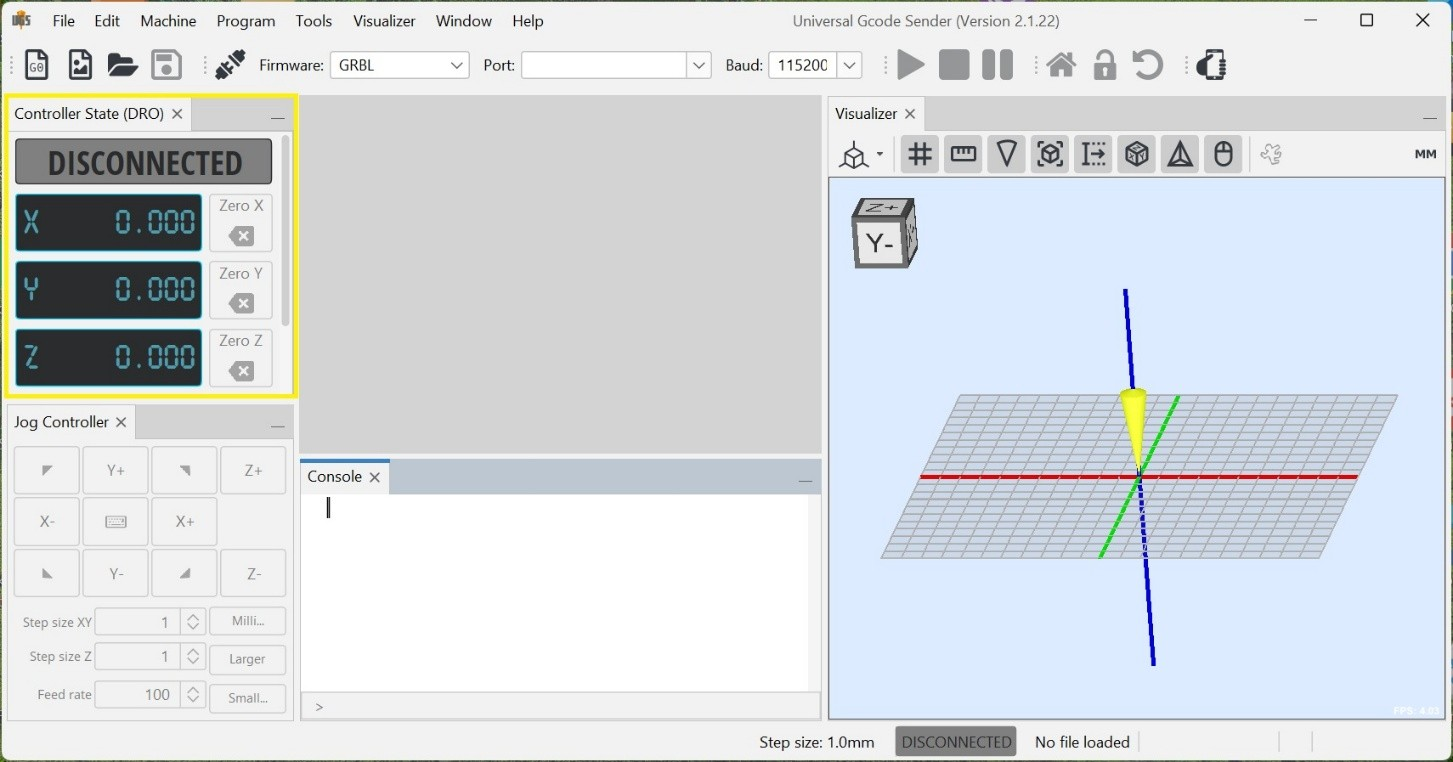
\includegraphics[width=0.85\linewidth]{../../Images/UGS/UGS_DRO}
	\caption{Controller State (DRO) -- Positionsanzeige in UGS}
	\label{fig:ugs_dro}
\end{figure}

\subsection{Zusammenspiel der Bedienbereiche}

Die genannten Bereiche arbeiten im praktischen Betrieb eng zusammen. Während die Jog Control zur manuellen Positionierung genutzt wird, erlaubt das DRO die unmittelbare Kontrolle der erreichten Koordinaten. Gleichzeitig zeigt die Console, welche Befehle an die Firmware übermittelt werden und wie diese darauf reagiert. Der Visualizer ergänzt diese Informationen durch die grafische Darstellung des geplanten beziehungsweise laufenden Bewegungsablaufs.

\begin{figure}[H]
	\centering
	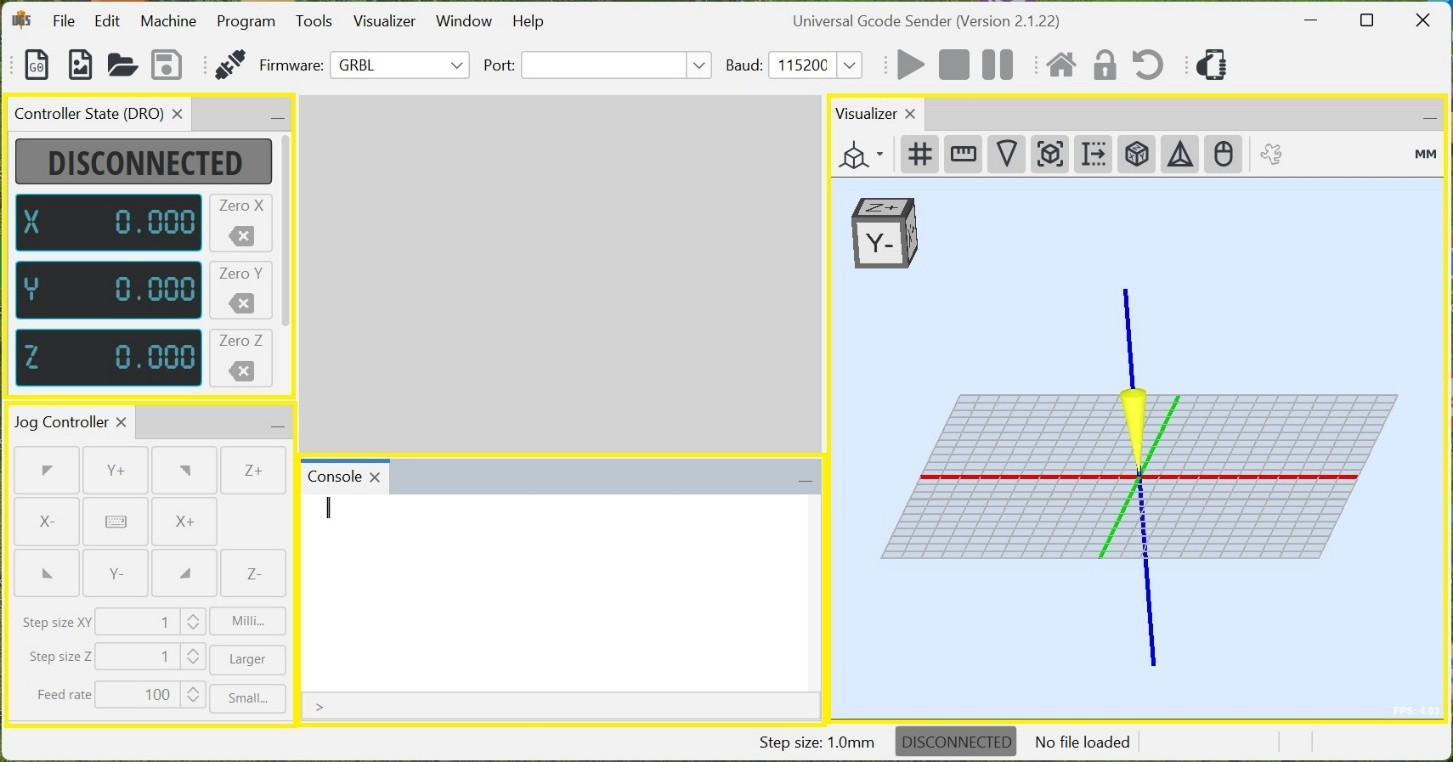
\includegraphics[width=0.85\linewidth]{../../Images/UGS/UGS_Anzeigen}
	\caption{Übersicht über die Bedien- und Anzeigefelder in UGS}
	\label{fig:ugs_anzeigen}
\end{figure}

\section{Installation des Universal G-Code Senders}

\subsection{Systemvoraussetzungen}

\begin{itemize}
	\item Betriebssystem: Windows 10 oder Windows 11, Linux oder macOS,
	\item Arbeitsspeicher: mindestens 2 GB RAM, empfohlen 4 GB RAM,
	\item Festplattenspeicher: mindestens 200 MB freier Speicherplatz,
	\item Schnittstelle: USB-Anschluss zur Verbindung mit der CNC-Maschine,
	\item USB-Treiber: abhängig vom verbauten USB-Chip des Controllers, zum Beispiel CH340 oder CP210x.
\end{itemize}

\subsection{Download und Installation}

Der Download erfolgt über die offizielle Download-Seite des Projekts beziehungsweise über die GitHub-Releases-Seite. Dort wird die aktuelle stabile Version ausgewählt und die für das jeweilige Betriebssystem passende Variante heruntergeladen, zum Beispiel \PYTHON{ugs-platform-app-win-x64.zip} für Windows 64-Bit \cite{ugs:github}.

Die Installation erfolgt in folgenden Schritten:

\begin{enumerate}
	\item Das heruntergeladene ZIP-Archiv in ein Verzeichnis eigener Wahl entpacken.
	\item In den entpackten Ordner wechseln.
	\item Den Unterordner \PYTHON{bin} öffnen.
	\item Die Anwendung durch Doppelklick auf \PYTHON{ugsplatform64.exe} starten.
	\item Eine mögliche Windows-Sicherheitswarnung über \emph{Weitere Informationen} und \emph{Trotzdem ausführen} bestätigen.
\end{enumerate}

\subsection{Erstverbindung mit der CNC-Maschine}

\begin{enumerate}
	\item Den Arduino beziehungsweise Controller über USB mit dem Computer verbinden.
	\item Im Windows-Geräte-Manager den zugewiesenen COM-Port unter \emph{Anschlüsse (COM \& LPT)} ermitteln.
	\item In UGS den ermittelten COM-Port im Dropdown-Menü \emph{Port} auswählen.
	\item Die Baudrate auf \PYTHON{115200} einstellen, da dies der Standard für GRBL v1.1 ist.
	\item Auf \emph{Connect} klicken.
	\item Bei erfolgreicher Verbindung erscheint im Konsolenfenster die GRBL-Versionsmeldung, zum Beispiel \PYTHON{Grbl 1.1h ['\$' for help]}.
	\item Als Erfolgstest kann der Befehl \PYTHON{\$\$} eingegeben und die ausgegebenen Parameter überprüft werden.
\end{enumerate}

\section{Konfiguration und Diagnose in UGS}

Die serielle Verbindung zwischen UGS und dem GRBL-Controller wird über den Port, die Baudrate und weitere Verbindungsparameter eingerichtet. Für GRBL v1.1 wird normalerweise eine Baudrate von \PYTHON{115200} Baud verwendet. Die Datenübertragung erfolgt mit 8 Datenbits, 1 Stoppbit und ohne Parität. Diese Konfiguration wird auch als \PYTHON{8N1} bezeichnet.

Für Diagnosezwecke können über die Console Status- und Steuerbefehle gesendet werden. Mit \PYTHON{?} wird der aktuelle Maschinenstatus abgefragt. Über \PYTHON{\$G} können die aktiven modalen G-Code-Zustände angezeigt werden. Die Eingabe von \PYTHON{\$I} gibt Versions- und Build-Informationen der Firmware aus. Fehlermeldungen und Alarmzustände werden ebenfalls in der Console angezeigt und können dort ausgewertet werden.

\section{Verwendung}

\subsection{G-Code selbst schreiben}

G-Code ist die Programmiersprache für numerisch gesteuerte Maschinen. In UGS können G-Code-Befehle entweder einzeln im Kommandozeilenfeld eingegeben oder als vollständige Datei geladen und im Batch-Mode ausgeführt werden \cite{ugs:github}.

\begin{longtable}{p{0.22\linewidth}p{0.68\linewidth}}
	\caption{Häufig verwendete G- und M-Codes}\label{tab:gcode_befehle}\\
	\hline
	Befehl & Funktion \\
	\hline
	\endfirsthead
	\hline
	Befehl & Funktion \\
	\hline
	\endhead
	\hline
	\endfoot
	\PYTHON{G0} & Eilgang beziehungsweise nicht bearbeitende Bewegung mit maximaler Geschwindigkeit \\
	\PYTHON{G1} & Linearinterpolation mit programmiertem Vorschub \\
	\PYTHON{G2} / \PYTHON{G3} & Kreisinterpolation im beziehungsweise gegen den Uhrzeigersinn \\
	\PYTHON{G20} / \PYTHON{G21} & Umschaltung zwischen Zoll- und Millimeter-Modus \\
	\PYTHON{G90} / \PYTHON{G91} & Absolutes beziehungsweise inkrementales Koordinatensystem \\
	\PYTHON{G28} & Fahrt zur vordefinierten Referenzposition \\
	\PYTHON{M3} / \PYTHON{M5} & Spindel oder Laser einschalten beziehungsweise ausschalten \\
	\PYTHON{M2} / \PYTHON{M30} & Programmende \\
	\PYTHON{F} & Vorschubgeschwindigkeit in mm/min \\
	\PYTHON{S} & Spindeldrehzahl oder Leistung bezogen auf den eingestellten Maximalwert \\
\end{longtable}

Das folgende Listing zeigt ein Beispielprogramm zur Abfahrt einer rechteckigen Kontur.

\begin{lstlisting}[caption={Beispielprogramm zur Abfahrt einer rechteckigen Kontur},label={lst:gcode_rechteck}]
	; Initialisierung
	G21        ; Metrischer Modus (mm)
	G90        ; Absolutes Koordinatensystem
	G17        ; XY-Ebene waehlen
	
	; Startposition anfahren
	G0 X0 Y0 Z5    ; Eilgang zur Startposition (Z5 mm Sicherheitshoehe)
	M3 S1000       ; Spindel einschalten (1000 RPM)
	
	; Eintauchen
	G1 Z-1 F100    ; Eintauchen auf Z-1 mm mit Vorschub 100 mm/min
	
	; Rechteckige Kontur (50 mm x 50 mm)
	G1 X50 Y0  F300    ; Seite 1
	G1 X50 Y50 F300    ; Seite 2
	G1 X0  Y50 F300    ; Seite 3
	G1 X0  Y0  F300    ; Zurueck zum Ursprung
	
	; Werkzeug anheben und Programm beenden
	G0 Z5      ; Werkzeug auf Sicherheitshoehe
	M5         ; Spindel ausschalten
	M2         ; Programmende
\end{lstlisting}

\subsection{G-Code-Datei importieren}

Für die maschinelle Fertigung wird G-Code typischerweise mit CAM-Software aus einem CAD-Modell generiert und als Datei exportiert. UGS unterstützt unter anderem die Dateiformate \PYTHON{.nc}, \PYTHON{.gcode}, \PYTHON{.txt} und \PYTHON{.tap} \cite{ugs:github}.

Der Importprozess in UGS erfolgt schrittweise:

\begin{enumerate}
	\item Datei über \emph{File} und \emph{Open} öffnen.
	\item Im Datei-Dialog die G-Code-Datei auswählen und mit \emph{Öffnen} bestätigen.
	\item UGS lädt und analysiert die Datei.
	\item Im Visualizer-Fenster wird der Werkzeugpfad als 2D/3D-Grafik dargestellt.
	\item Vor dem Start den Werkzeug-Nullpunkt beziehungsweise Werkstück-Ursprung an der Maschine definieren und in UGS über \emph{Zero All} zurücksetzen.
	\item Maschinenstatus auf \PYTHON{Idle} prüfen.
	\item Die Übertragung durch Klick auf die Play-Schaltfläche beziehungsweise \emph{Send File} starten.
	\item Die Befehle werden im Batch-Mode sequenziell an die Maschine übermittelt.
\end{enumerate}
